\documentclass{standalone}
\usepackage{tikz}
\usetikzlibrary{patterns, positioning}


\begin{document}
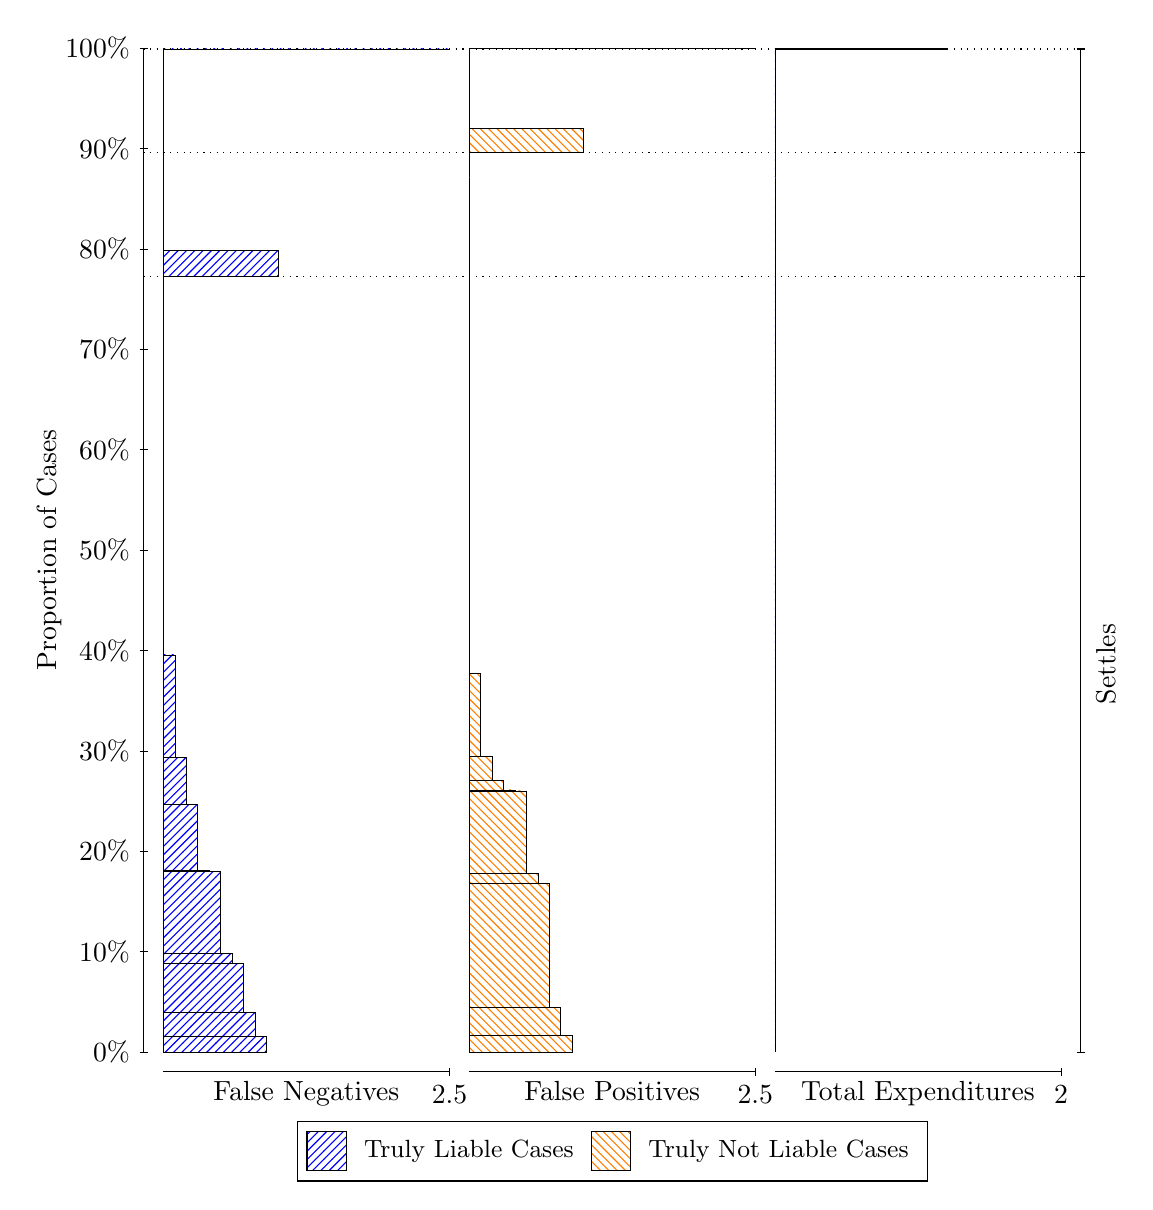
\begin{tikzpicture}
\draw[black, very thin] (1.5,1.75) -- (1.5,14.5);
\node[rotate=90, text=black, anchor=center] at (0.3, 8.125) {Proportion of Cases};
\draw[black, very thin] (1.45,1.75) -- (1.55,1.75);
\node[text=black, anchor=east] at (1.45, 1.75) {0\%};
\draw[black, very thin] (1.45,3.025) -- (1.55,3.025);
\node[text=black, anchor=east] at (1.45, 3.025) {10\%};
\draw[black, very thin] (1.45,4.3) -- (1.55,4.3);
\node[text=black, anchor=east] at (1.45, 4.3) {20\%};
\draw[black, very thin] (1.45,5.575) -- (1.55,5.575);
\node[text=black, anchor=east] at (1.45, 5.575) {30\%};
\draw[black, very thin] (1.45,6.85) -- (1.55,6.85);
\node[text=black, anchor=east] at (1.45, 6.85) {40\%};
\draw[black, very thin] (1.45,8.125) -- (1.55,8.125);
\node[text=black, anchor=east] at (1.45, 8.125) {50\%};
\draw[black, very thin] (1.45,9.4) -- (1.55,9.4);
\node[text=black, anchor=east] at (1.45, 9.4) {60\%};
\draw[black, very thin] (1.45,10.675) -- (1.55,10.675);
\node[text=black, anchor=east] at (1.45, 10.675) {70\%};
\draw[black, very thin] (1.45,11.95) -- (1.55,11.95);
\node[text=black, anchor=east] at (1.45, 11.95) {80\%};
\draw[black, very thin] (1.45,13.225) -- (1.55,13.225);
\node[text=black, anchor=east] at (1.45, 13.225) {90\%};
\draw[black, very thin] (1.45,14.5) -- (1.55,14.5);
\node[text=black, anchor=east] at (1.45, 14.5) {100\%};

\draw[black, very thin] (13.4,1.75) -- (13.4,14.5);
\draw[black, very thin] (13.35,1.75) -- (13.45,1.75);
\node[anchor=west] at (13.35, 1.75) {};
\draw[black, very thin] (13.35,11.603) -- (13.45,11.603);
\node[anchor=west] at (13.35, 11.603) {};
\draw[black, very thin] (13.35,13.177) -- (13.45,13.177);
\node[anchor=west] at (13.35, 13.177) {};
\draw[black, very thin] (13.35,14.488) -- (13.45,14.488);
\node[anchor=west] at (13.35, 14.488) {};
\draw[black, very thin] (13.35,14.494) -- (13.45,14.494);
\node[anchor=west] at (13.35, 14.494) {};
\draw[black, very thin] (13.35,14.5) -- (13.45,14.5);
\node[anchor=west] at (13.35, 14.5) {};

\draw[black, very thin, pattern color=blue, pattern=north east lines] (1.75,1.75) rectangle (3.058,1.9436);
\draw[black, very thin, pattern color=blue, pattern=north east lines] (1.75,1.9436) rectangle (2.9127,2.2566);
\draw[black, very thin, pattern color=blue, pattern=north east lines] (1.75,2.2566) rectangle (2.7673,2.8749);
\draw[black, very thin, pattern color=blue, pattern=north east lines] (1.75,2.8749) rectangle (2.622,2.9974);
\draw[black, very thin, pattern color=blue, pattern=north east lines] (1.75,2.9974) rectangle (2.4767,4.0468);
\draw[black, very thin, pattern color=blue, pattern=north east lines] (1.75,4.0468) rectangle (2.3313,4.0581);
\draw[black, very thin, pattern color=blue, pattern=north east lines] (1.75,4.0581) rectangle (2.186,4.8955);
\draw[black, very thin, pattern color=blue, pattern=north east lines] (1.75,4.8955) rectangle (2.0407,5.4913);
\draw[black, very thin, pattern color=blue, pattern=north east lines] (1.75,5.4913) rectangle (1.8953,6.7916);
\draw[black, very thin, pattern color=orange, pattern=north west lines] (1.75,6.7916) rectangle (1.75,11.603);
\draw[black, very thin, pattern color=blue, pattern=north east lines] (1.75,11.603) rectangle (3.2033,11.926);
\draw[black, very thin, pattern color=orange, pattern=north west lines] (1.75,11.926) rectangle (1.75,13.177);
\draw[black, very thin, pattern color=orange, pattern=north west lines] (1.75,13.177) rectangle (1.75,13.484);
\draw[black, very thin, pattern color=blue, pattern=north east lines] (1.75,13.484) rectangle (1.75,14.488);
\draw[black, very thin, pattern color=blue, pattern=north east lines] (1.75,14.488) rectangle (5.3833,14.49);
\draw[black, very thin, pattern color=orange, pattern=north west lines] (1.75,14.49) rectangle (1.75,14.494);
\draw[black, very thin, pattern color=orange, pattern=north west lines] (1.75,14.494) rectangle (1.75,14.496);
\draw[black, very thin, pattern color=blue, pattern=north east lines] (1.75,14.496) rectangle (1.75,14.5);
\draw[black, very thin, pattern color=orange, pattern=north west lines] (5.6333,1.75) rectangle (6.9413,1.9604);
\draw[black, very thin, pattern color=orange, pattern=north west lines] (5.6333,1.9604) rectangle (6.796,2.319);
\draw[black, very thin, pattern color=orange, pattern=north west lines] (5.6333,2.319) rectangle (6.6507,3.8945);
\draw[black, very thin, pattern color=orange, pattern=north west lines] (5.6333,3.8945) rectangle (6.5053,4.017);
\draw[black, very thin, pattern color=orange, pattern=north west lines] (5.6333,4.017) rectangle (6.36,5.0664);
\draw[black, very thin, pattern color=orange, pattern=north west lines] (5.6333,5.0664) rectangle (6.2147,5.0777);
\draw[black, very thin, pattern color=orange, pattern=north west lines] (5.6333,5.0777) rectangle (6.0693,5.196);
\draw[black, very thin, pattern color=orange, pattern=north west lines] (5.6333,5.196) rectangle (5.924,5.5081);
\draw[black, very thin, pattern color=orange, pattern=north west lines] (5.6333,5.5081) rectangle (5.7787,6.5615);
\draw[black, very thin, pattern color=blue, pattern=north east lines] (5.6333,6.5615) rectangle (5.6333,11.603);
\draw[black, very thin, pattern color=orange, pattern=north west lines] (5.6333,11.603) rectangle (5.6333,12.854);
\draw[black, very thin, pattern color=blue, pattern=north east lines] (5.6333,12.854) rectangle (5.6333,13.177);
\draw[black, very thin, pattern color=orange, pattern=north west lines] (5.6333,13.177) rectangle (7.0867,13.484);
\draw[black, very thin, pattern color=blue, pattern=north east lines] (5.6333,13.484) rectangle (5.6333,14.488);
\draw[black, very thin, pattern color=orange, pattern=north west lines] (5.6333,14.488) rectangle (5.6333,14.492);
\draw[black, very thin, pattern color=blue, pattern=north east lines] (5.6333,14.492) rectangle (5.6333,14.494);
\draw[black, very thin, pattern color=orange, pattern=north west lines] (5.6333,14.494) rectangle (9.2667,14.496);
\draw[black, very thin, pattern color=blue, pattern=north east lines] (5.6333,14.496) rectangle (7.8133,14.5);
\draw[black, very thin, pattern color=orange, pattern=north west lines] (9.5167,1.75) rectangle (9.5167,6.5615);
\draw[black, very thin, pattern color=blue, pattern=north east lines] (9.5167,6.5615) rectangle (9.5167,11.603);
\draw[black, very thin, pattern color=orange, pattern=north west lines] (9.5167,11.603) rectangle (9.5167,12.854);
\draw[black, very thin, pattern color=blue, pattern=north east lines] (9.5167,12.854) rectangle (9.5167,13.177);
\draw[black, very thin, pattern color=orange, pattern=north west lines] (9.5167,13.177) rectangle (9.5167,13.484);
\draw[black, very thin, pattern color=blue, pattern=north east lines] (9.5167,13.484) rectangle (9.5167,14.488);
\draw[black, very thin, pattern color=orange, pattern=north west lines] (9.5167,14.488) rectangle (11.697,14.492);
\draw[black, very thin, pattern color=blue, pattern=north east lines] (9.5167,14.492) rectangle (11.697,14.494);
\draw[black, very thin, pattern color=orange, pattern=north west lines] (9.5167,14.494) rectangle (11.697,14.496);
\draw[black, very thin, pattern color=blue, pattern=north east lines] (9.5167,14.496) rectangle (11.697,14.5);
\draw[black, dotted] (1.5,11.603) -- (13.4,11.603);
\draw[black, dotted] (1.5,13.177) -- (13.4,13.177);
\draw[black, dotted] (1.5,14.488) -- (13.4,14.488);
\draw[black, dotted] (1.5,14.494) -- (13.4,14.494);
\draw[black, very thin] (1.75,1.5) -- (5.3833,1.5);
\node[text=black, anchor=north] at (3.5667, 1.5) {False Negatives};
\draw[black, very thin] (5.3833,1.45) -- (5.3833,1.55);
\node[text=black, anchor=north] at (5.3833, 1.45) {2.5};

\draw[black, very thin] (5.6333,1.5) -- (9.2667,1.5);
\node[text=black, anchor=north] at (7.45, 1.5) {False Positives};
\draw[black, very thin] (9.2667,1.45) -- (9.2667,1.55);
\node[text=black, anchor=north] at (9.2667, 1.45) {2.5};

\draw[black, very thin] (9.5167,1.5) -- (13.15,1.5);
\node[text=black, anchor=north] at (11.333, 1.5) {Total Expenditures};
\draw[black, very thin] (13.15,1.45) -- (13.15,1.55);
\node[text=black, anchor=north] at (13.15, 1.45) {2};

\node[text=black, centered, rotate=90] at (13.72, 6.6765) {Settles};





\draw (7.449999999999999,1.5) node[draw=none] (baseCoordinate) {};
\begin{scope}[align=center]
        \matrix[scale=0.5, draw=black, below=0.5cm of baseCoordinate, nodes={draw}, column sep=0.1cm]{
            \node[rectangle, draw, minimum width=0.5cm, minimum height=0.5cm, pattern color=blue, pattern=north east lines] {}; &
            \node[draw=none, font=\small, text=black] (B) {Truly Liable Cases}; &
            \node[rectangle, draw, minimum width=0.5cm, minimum height=0.5cm, pattern color=orange, pattern=north west lines] {}; &
            \node[draw=none, font=\small, text=black] (B) {Truly Not Liable Cases}; \\
            };
\end{scope}

\end{tikzpicture}
\end{document}